\documentclass{standalone}
\usepackage{pgfplots}
\pgfplotsset{compat=1.18}

\begin{document}
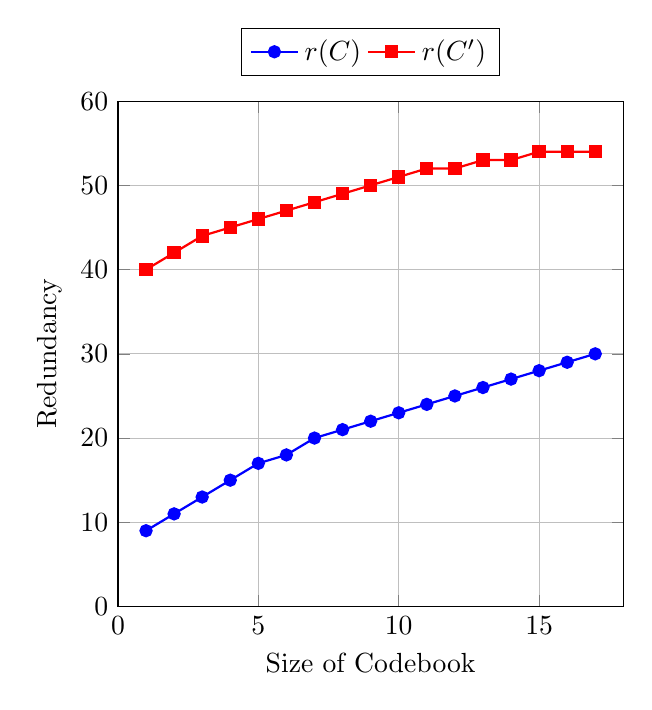
\begin{tikzpicture}
\begin{axis}[
    width=8cm,
    height=8cm,
    xlabel={Size of Codebook},
    ylabel={Redundancy},
    legend style={at={(0.5,1.05)}, anchor=south},
    legend columns=2,
    grid=major,
    xmin=0, xmax=18,
    ymin=0, ymax=60,
    xtick={0, 5, 10, 15},
    ytick={0, 10, 20, 30, 40, 50, 60},
]

% Data for r(C)
\addplot[
    color=blue,
    mark=*,
    thick,
    ]
    coordinates {
    (1,9) (2,11) (3,13) (4,15) (5,17) (6,18) (7,20) (8,21) (9,22) (10,23)
    (11,24) (12,25) (13,26) (14,27) (15,28) (16,29) (17,30)
    };

% Data for r(C')
\addplot[
    color=red,
    mark=square*,
    thick,
    ]
    coordinates {
    (1,40) (2,42) (3,44) (4,45) (5,46) (6,47) (7,48) (8,49) (9,50) (10,51)
    (11,52) (12,52) (13,53) (14,53) (15,54) (16,54) (17,54)
    };

\legend{$r(C)$, $r(C')$}
\end{axis}
\end{tikzpicture}
\end{document}